\documentclass{beamer}
\usetheme{Madrid}
\usepackage{circuitikz}
\usepackage{tikz}
\usepackage{amsmath}
\usepackage{graphics}
%\usepackage{xcolor}
\renewcommand{\bibname}{References}
\author{\bf{AC }}
\institute{Research Group-Nepal}
\logo{\Huge\color{red} $\star$ 	\Huge\color{violet} $\star$}
\title[ACRGN]{\Huge\bf{ACRGN}}
	\subtitle{A Presentation}
	\date{\today}
	\begin{document}
		
		
		\begin{frame}
	\begin{center}
%		{	\frametitle{\hspace{1.5cm}\Huge\bf{\Huge A Discussion program on}} \\[0.3cm] \color{blue}\Huge \bf \color{red} Physics Computing Skill\\ \color{blue}Development Program in \color{red} Nepal   \\\color{blue}}\\[0.3cm]
		\Huge\color{red} $\star$ \hspace{0.5cm}\color{orange} $\star$ \hspace{0.5cm}	\Huge\color{yellow} $\star$ \hspace{0.5cm} \Huge\color{green} $\star$ \hspace{0.5cm} \Huge\color{blue} $\star$  \hspace{0.5cm} \Huge\color{indigo} $\star$ \hspace{0.5cm} \Huge\color{violet} $\star$ \\
		\vspace{0.3cm}
%				%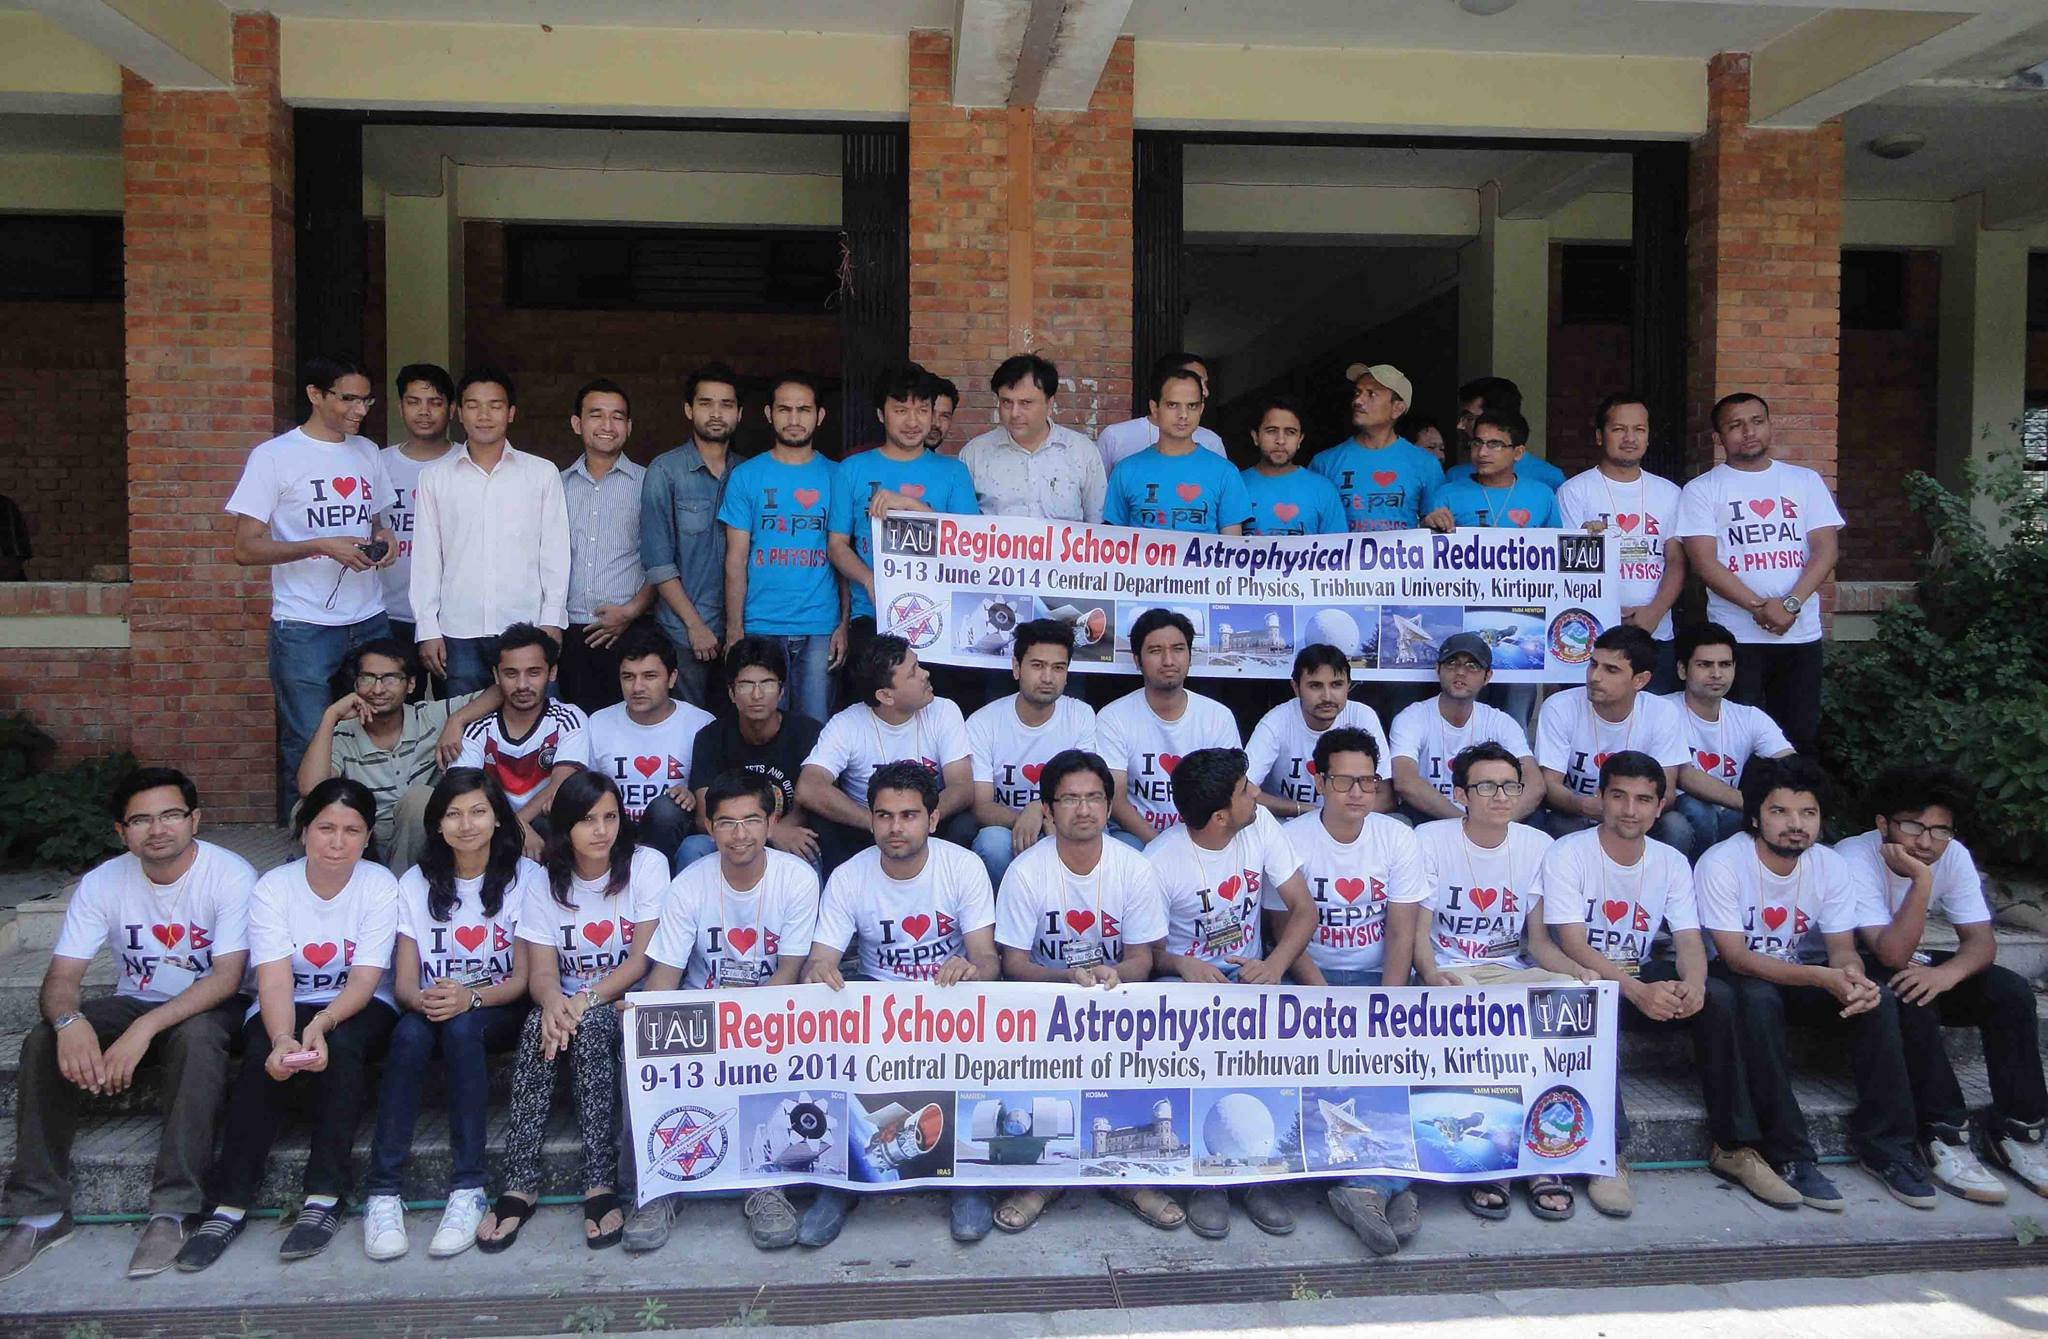
\includegraphics[height=3cm]{A}
%				%	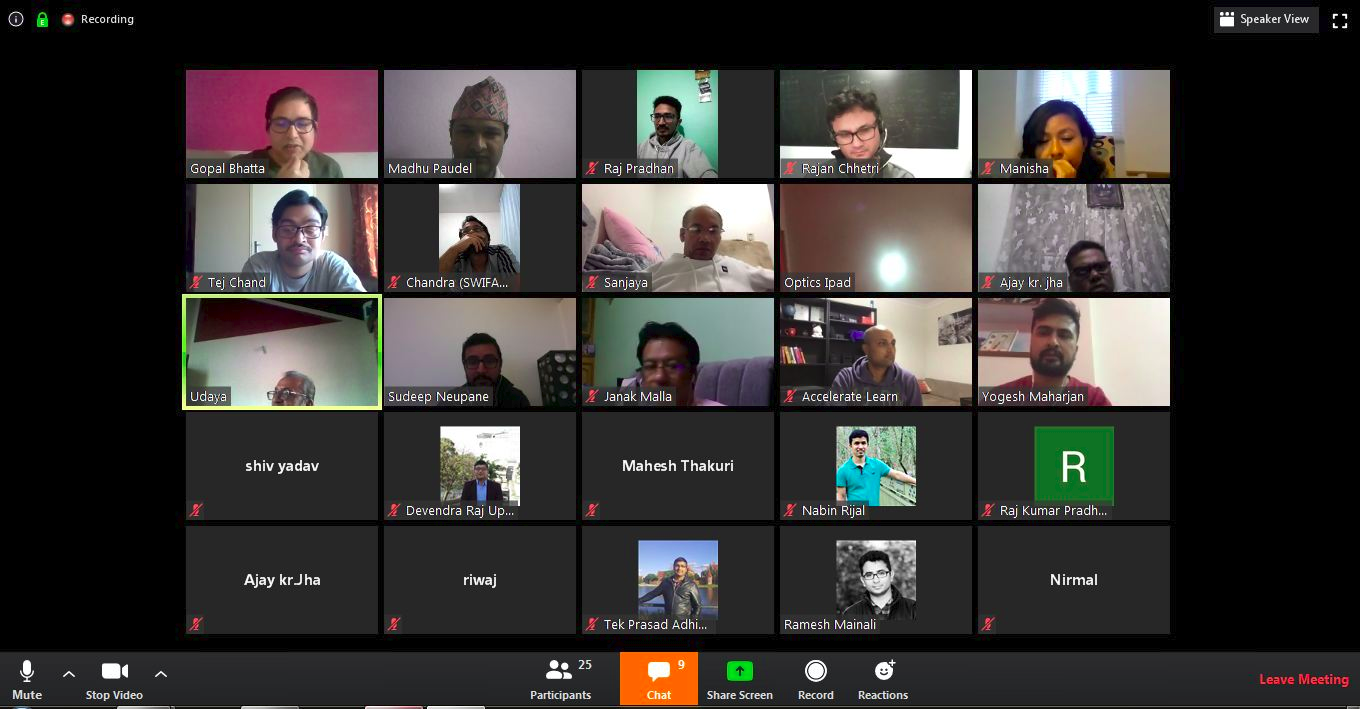
\includegraphics[height=3cm]{21}\\
%%					
						{\color{blue}\Huge \bf  NPS School of \color{red} Computing\\[0.2cm]}
	\Huge\color{red} $\star$ \hspace{0.5cm}\color{orange} $\star$ \hspace{0.5cm}	\Huge\color{yellow} $\star$ \hspace{0.5cm} \Huge\color{green} $\star$ \hspace{0.5cm} \Huge\color{blue} $\star$  \hspace{0.5cm} \Huge\color{indigo} $\star$ \hspace{0.5cm} \Huge\color{violet} $\star$ \\			
	\end{center}
		\end{frame}
%		
%	\begin{frame}
%\frametitle{\bf  Meeting 1}	
%\begin{enumerate}
%	\bf 
%\item \color{red}To discuss about the need of professional society of Astrophysics and Cosmology in Nepal. 
%\item \color{blue} To discuss about activities such as outreach, educational, research and collaboration.
%%\item \color{red} To discuss about need of a core team of experts and qualified professional who will pursue to carry out agenda 1 and 2.  
%\end{enumerate}
%	\end{frame}
%
%\begin{frame}
%\frametitle{\bf Meeting 1}
%\centering
%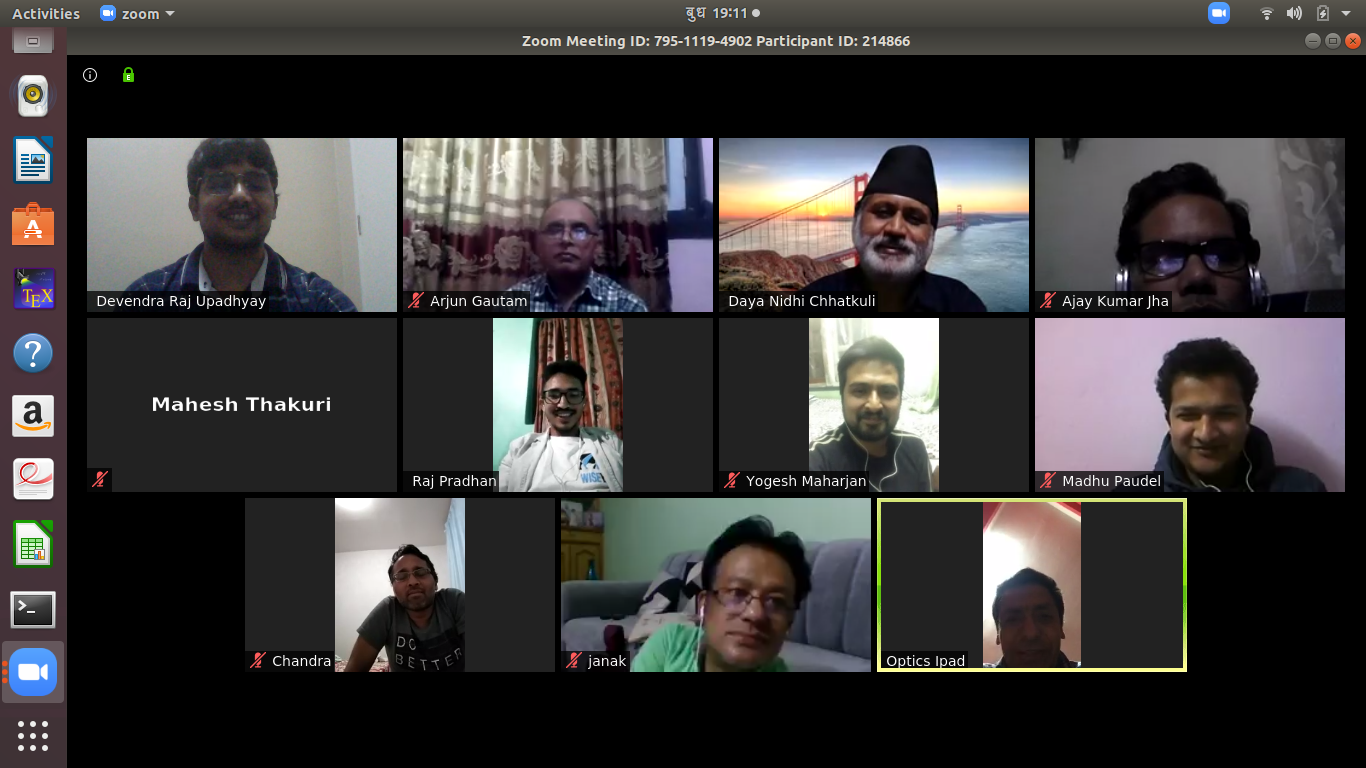
\includegraphics[width=12cm]{Astro}
%\end{frame}
%
%	\begin{frame}
%\frametitle{\bf  Meeting 1(Summary)}	
%\begin{enumerate}
%	\bf 
%\item \color{red}  How can we start our goal?
%First, starting from minor works like discussing weekly or monthly specific
%collaborative or individual research work papers via webinar. i.e. paper
%presentation. That means engaging in regular talks (Main emphasis).
%\item \color{blue} Concept of professional society of Astrophysics and Cosmology in Nepal
%that can manage education, research and collaboration.
%\item \color{red} Have to fully focus on research based programs i.e. our plan should be
%directed on research.
%\item \color{blue}How can we fulfill the gap between senior and young researchers?
%
%\end{enumerate}
%\end{frame}
%
%	\begin{frame}
%\frametitle{\bf  Meeting 1(Summary)}	
%\begin{enumerate}
%	\bf 
%	\item \color{red} Identify the collaborators and research grants institutes like International
%	Astronomical Union(IAU), CAS(Chinese Academy of Science), American
%	Astronomical Society(AAS), Korean Astronomical Society(KAS),
%	University Centre for Astronomy and Astrophysics (IUCAA), University
%	Grants Commissions(UGC) Nepal, Nepal Academy of Science and
%	Technology (NAST), Nepal, etc and to put forward research exchange
%	policies like Nepal - China Funding Program on Astrophysics and
%	Astronomy with resource persons.
%	\item \color{blue} To connect with international experts, starting first from Nepali experts
%	and then others.
%	\item \color{red} Create a Journal Club on Slack, for weekly interaction with senior school
%	students and to the public!
%	
%\end{enumerate}
%\end{frame}
%
%	\begin{frame}
%\frametitle{\bf  Meeting 1(Summary)}	
%\begin{enumerate}
%	\bf 
%
%	\item \color{red} For skill and knowledge, we can conduct yearly Summer School or
%	Winter school.9. To search the way of our nation and our professionals can get
%	membership of International Astronomical Union(IAU).
%	\item \color{blue} Starting from minor programs like interaction such that we would
%	maintain Energy to meet our target, i.e fully functional research body or
%	society.
%	\item \color{red} Should maintain a research bridge between BSc to MSc to PhD. For
%	BSc, try to open a scholarship scheme!
%	\item \color{blue} Requested and purposed research Room (CDP astrophysics LAB) or
%	others??
%	\item \color{red} Open access for all Nepali researchers in Astrophysics and
%	Cosmology !!!
%	\item \color{blue} Out of political interference!
%	
%\end{enumerate}
%\end{frame}
%
%\begin{frame}
%\frametitle{\bf Discussion Topics}
%\begin{itemize}
%	\bf 
%	\item \color{blue} We shared our ideas and opinions on Functionality and Working Modality of this group
%	\item \color{red} Brain stroming on need of this type group 
%\end{itemize}
%\end{frame}
%
%\begin{frame}
%\frametitle{\bf Meeting 2}
%\centering
%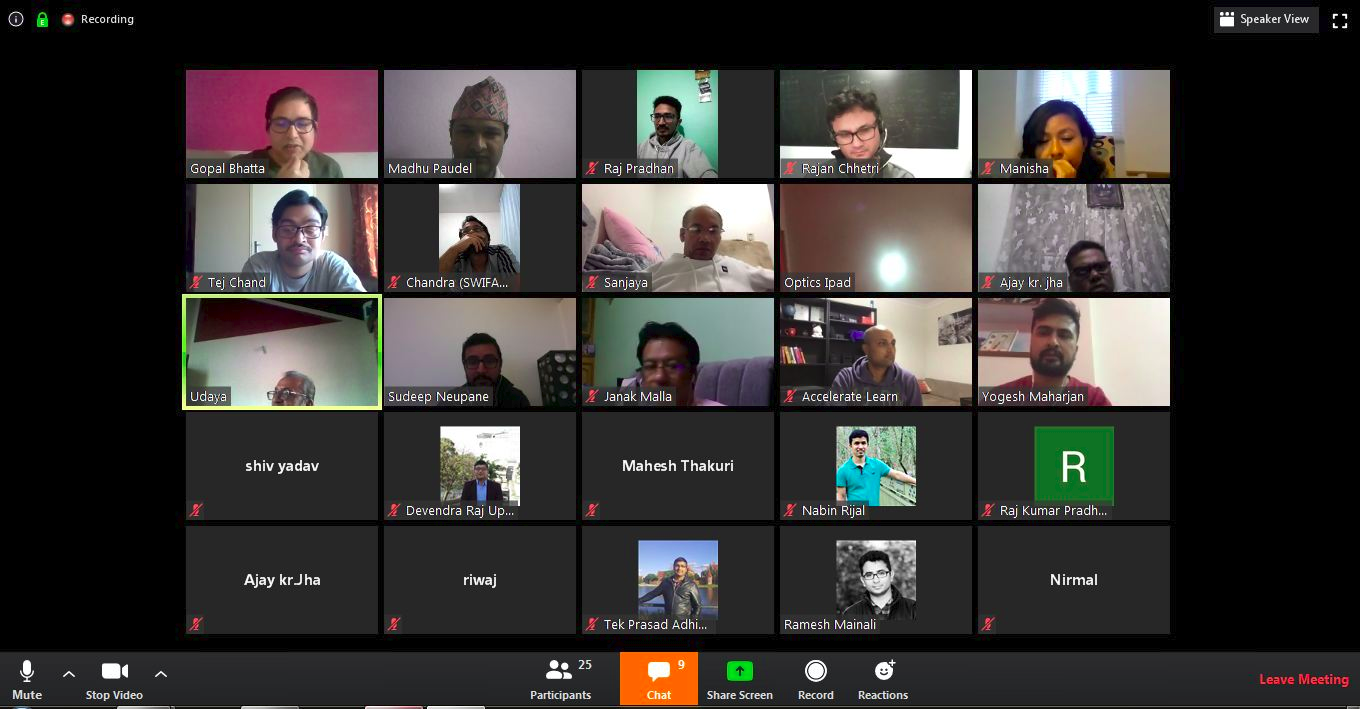
\includegraphics[width=12cm]{21}
%\end{frame}
%\begin{frame}
%\frametitle{\bf Meeting 2}
%\centering
%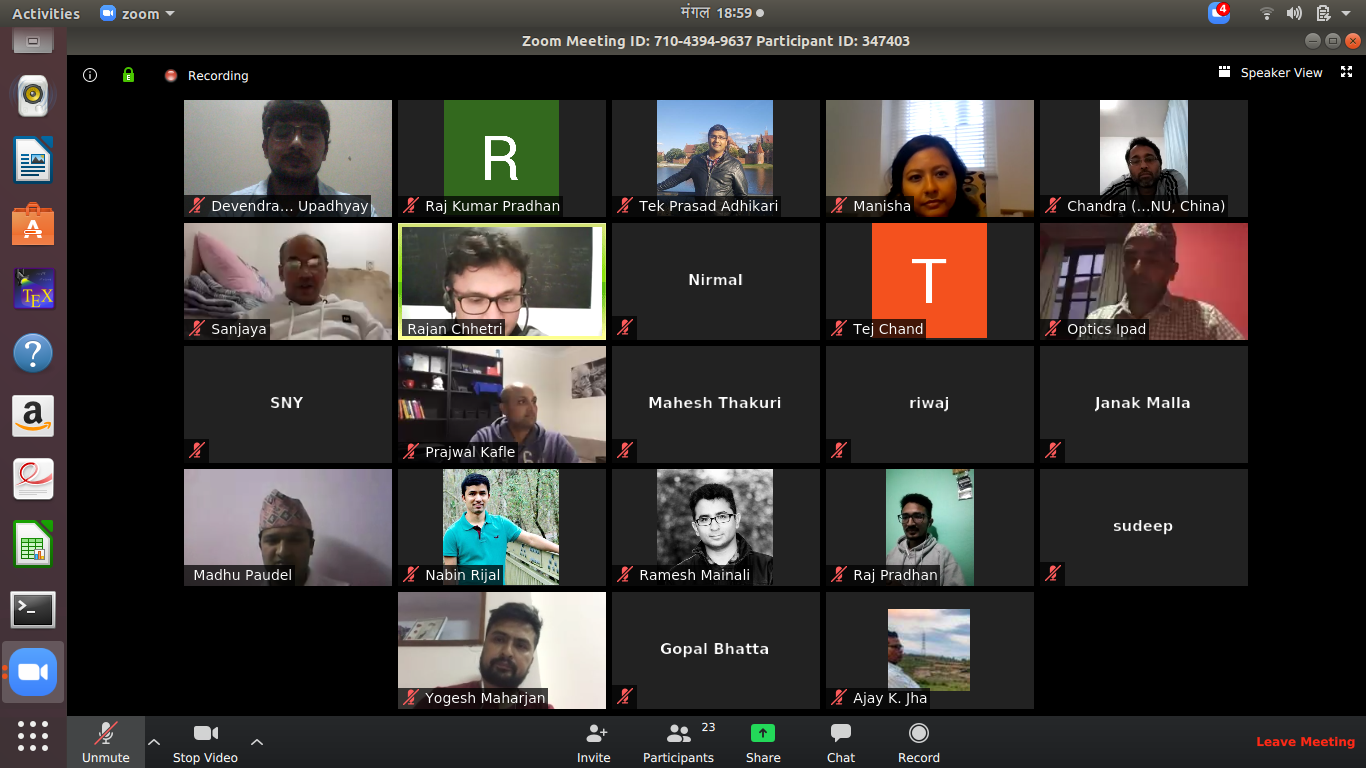
\includegraphics[width=12cm]{2}
%\end{frame}
%
%
%\begin{frame}
%\frametitle{\bf Summaries }
%
%\color{red} \bf 
%\begin{itemize}
%\item \color{blue} Dr. Ajay Sir, Dr Shiva Sir, Dr. Arjun Sir, Bhanu Bhakta Sir, Dayanidhi Sir, Janak Sir are highly interested to collaborate for further researches in coming days with abroad seniors and scientists as well in order to enhance professional development in this field. 
%\item \color{red} This group will act as contact point or bridging for collaborative research, discussion and skill building - Dr. Sanjay Paudel, Dr. Gopal Bhatta, Dr. Prajwal Kafle, Dr. Manisha Shrestha
%\item \color{blue}This group will provide good exposure for enthusiast young in field of astronomy, astrophysics and cosmology - Dr. Riwaj Pokharel 
%This group will be a platform for discussion journals, webinars - Dr. Chandra Bahadur Singh
%\end{itemize}
%
%\end{frame}
%\begin{frame}
%\frametitle{\bf Summaries (cont..) }
%\begin{itemize}
%	\bf 
%	\item \color{red} We need further quality discussions and idea sharing for exploring need of this type of group, from those discussions we can project (seting big dream - (like) within 20-30yrs building infrastructure for quality scientifc research and exploring resources, funding for continuing institutional development ) -  Dr. Sudeep Neupane
%	
%	
%	\item \color{blue} This group will facililate mentorship for proposal writing, honing academic research skills and provide international exposure as well. - Dr. Rajan Chhetri
%	
%	\item \color{red}  Dr. T.P. Adhikari, Dr. Nabin Rijal, Tej Chand had committed to help further development of this group/scoiety through ideas, opinions and skills 
%	
%
%\end{itemize}
%
%\end{frame}
%
%
%
%\begin{frame}
%\frametitle{\bf Summaries (cont..) }
%\begin{itemize} 
%	\bf 
%	
%	\item \color{blue}  For the certain time being this group will conduct futher zoom meetings and will discuss on functionality and working modality, regarding from yesterday's meeting
%	Researchs are carried out by individuals, if needed this type group go ahead and best wishes - Prof. Dr. Udayaraj Khanal Sir
%	
%	\item \color{red}  We all are agreed that this group will not compete existing societies and other personalities, won't do political doctorine or groupism, we are ready to encompass with existing Research Departments (Sepeical CDP), societies (NPS, NASO ..) and others, if needed for further developement of scientific knowlege. 
%\end{itemize}
%
%\end{frame}
%\begin{frame}
%\frametitle{\bf Take Care, Stay Safe \& Stay busy in Research}
%\centering
%
\includegraphics[width=10cm]{Thn}
%\end{frame}	
	
\end{document}

